\documentclass[twoside, openright]{RadboudReport}
\usepackage{amsmath}
\usepackage[english]{babel}         % Sets document language to English
\usepackage[sorting=none, style=ieee,backend=bibtex8]{biblatex} 
\bibliography{bibliography.bib} 
%\addbibresource}    % Define bibliography
\usepackage[hidelinks]{hyperref}    % Makes links in document clickable and adds
\usepackage{xspace}             
\usepackage{float}   % in your preamble                
                                    % the \href{}{} command to create hyperlinks
\newcommand{\adm}{\textsc{adm}\xspace}
\newcommand{\mots}{\textsc{mots}\xspace}
\newcommand{\mn}{{\mu\nu}}
\newcommand{\ab}{{\alpha\beta}}
\usepackage{mathrsfs}
\usepackage{tensor}
\usepackage{noindentafter}
\NoIndentAfterEnv{equation}
\NoIndentAfterEnv{equation*}
% title defines the title of your thesis as printed on the cover and as included in the meta data of the compiled pdf. the Radboud style guide advises to restrict this title to *at most* two lines in the compiled pdf.
\title{Apparent horizons in non-spherically symmetric Vaidya spacetimes}
% You can add extra information to your title by defining a subtitle inThesisSubtitle
\subtitle{Numerically finding Marginally Outer Trapped Surfaces (MOTSs) in different slicings of the spacetime}
% The supertitle defines text above the title. For thesis, this could (for example) be the type of thesis you are writing, both in its level (bachelor or master) and in the programme you are writing the thesis for. For example: "Bachelor thesis Physics and Astronomy"
\supertitle{Bachelor thesis Physics and Astronomy}
% The institute command is used to set the name of the institute that appears on the cover. Defining this is especially important when you did your internship externally.
\institute{Institute for Mathematics, Astrophysics and Particle Physics (IMAPP)}
% Don't forget to define your own name(s). We would very much like to know who did this excellent research :-)! \The template with print your name(s) in the left column on the cover.
\addnameleft{Ruud van Witzenburg}{Author}
% Define the names of supervisors and possibly other assessors of your work. These names will be printed on the cover in the column on the right.
\addnameright{Dr. Béatrice Bonga}{Supervisor \& First Assessor}
\addnameright{Prof. dr. Badri Krishnan}{Second Assessor}

% In date you define the date that should be printed on the cover of your thesis. If you set it to \today, the date at time of compilation will be used automatically. If you don't define the date, date will be printed on the cover.
\date{\today}
% coverabstract defines the text printed on the coverpage of your thesis. It should be short and to the point.
\coverabstract{Marginally Outer Trapped Surfaces (MOTSs) replace the concept of event horizons within numerical relativity due to their quasi-locality. In this thesis, we use a numerical algorithm, MOTSfinder, to examine the slicing dependence of Schwarzschild and ingoing Vaidya spacetimes. We find the location of the MOTSs in Schwarzschild to be independent of slicing, as expected. Furthermore, we explore the geometric properties of these MOTSs by expanding the shear and expansion into spherical harmonics. We find a nonzero shear for the outward null normal, motivating us to look at Lorentz boosts in Kerr-Schild coordinates and find an equivalence between slicings and boosts. We conclude by showing our nonzero shear as gauge radiation within our framework of Lorentz boosts and discussing some runtime issues and possible further research.}

\begin{document}

\maketitle
\cleardoublepage

\tableofcontents

\chapter{Introduction}

\section{The importance of MOTSs in numerical relativity}

In  general relativity, we use the concept of an event horizon to determine the 'boundary' of a black hole. The definition of an event horizon can be most easily explained using a conformal diagram of the Schwarzschild spacetime, as given in figure \ref{fig:Penrosediagramschwarzschild}.

\begin{figure}[!htb]
	\centering
	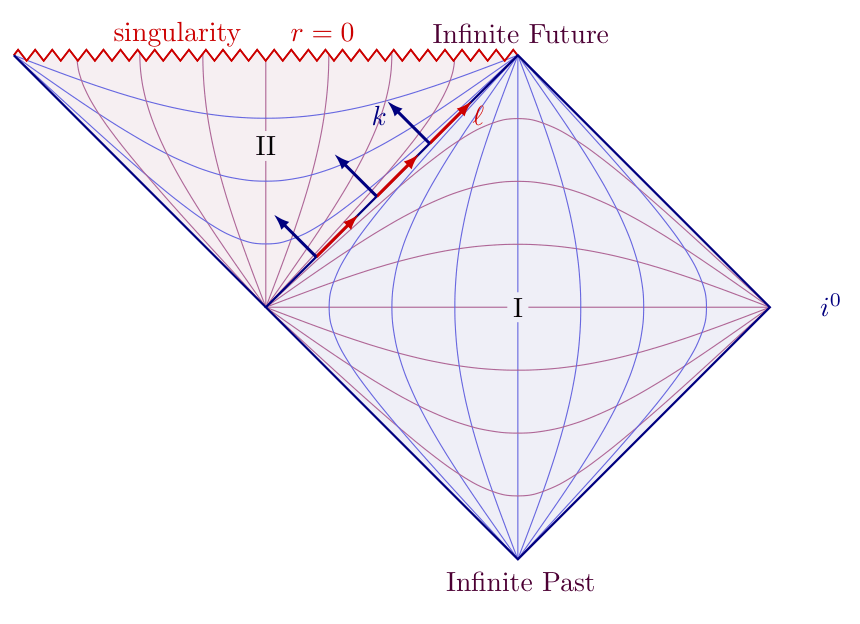
\includegraphics[width=0.8\textwidth]{Figures/penrose_diagram_schwarzschild-1.png}
	\caption{The conformal diagram for the Schwarzschild spacetime.}
	\label{fig:Penrosediagramschwarzschild}
\end{figure}

Region I denotes all of the universe visible to an observer outside the black hole, with the infinite time-like future and past at the top and bottom of the region, respectively. We have space-like infinity $i^0$ to the right of the region. Region II describes the interior of the black hole, with its singularity at $r = 0$, as we would expect. Any massive object or light would travel at an angle $\theta \leq 45^{\circ}$. Therefore it would be impossible to prevent an object reaching the singularity after it has passed the boundary between regions I and II. This is the event horizon of the black hole. \newline 

This immediately starts to cause trouble within our framework of numerical relativity, as it might not be the case that we have the metric for all times. Therefore, we are unable to look at the behavior of objects at future infinity and have no way to actually see if there is an event horizon or not. \newline

We use the concept of a marginally outer trapped surface (MOTS) to define the boundary of a black hole quasi-locally, which we will discuss in more detail in chapter \ref{chapter:theoreticalbackground}. MOTSs will always lie inside the event horizon of the black hole, or, in some cases like the stationary Schwarzschild black hole, will coincide with it. This motivates us to use MOTSs as the boundary of a black hole, and not the event horizon.\newline

\section{The dependency of the time-coordinate in finding MOTSs}

To find these MOTSs, we need to break up our four-dimensional metric into three spatial dimensions and one temporal dimension. We use the Arnowitt-Deser-Misner (ADM) formalism to expand our 4-dimensional spacetime into a 3+1-dimensional spacetime, defining a `time' coordinate $\tau$ that is constant along the 'slice' of our 3-dimensional space, or more formally, hypersurface. We then look for the MOTSs along these hypersurfaces of a certain time coordinate. This implicitly makes the shape of these MOTSs dependent on our choice of time coordinate.\newline

A good review of this effect can be found in a paper by Schnetter and Krishnan from 2006 \cite{badripaper}. This paper shows that the shape of the MOTS can be deformed in a non-spherically symmetric way despite Vaidya being spherically symmetric dependent on our choice of time coordinate. We will try to replicate these results to double-check our methods. \newline

After reproducing the results on the shape of the MOTS in Vaidya spacetimes in \cite{badripaper}, we will move on to studying not just the shape of the MOTS, but also its geometric properties, expanding our study to include the shear and expansion.

\chapter{Theoretical background}
\label{chapter:theoreticalbackground}

\section{General Relativity}

In general relativity, we describe gravity using curved spacetime. This theory works incredibly well, describing very subtle effects not accurately described by Newtonian gravity. Curved spacetimes are defined by the metric $g_\mn$, where $\mu$ and $\nu$ are the coordinates. As an example, flat spacetime, as used in special relativity, is described by

\begin{equation}
	g = 
	\begin{pmatrix}
		-1 & 0 & 0 & 0 \\
		0 & 1 & 0  & 0 \\
		0 & 0 & 1 & 0 \\
		0 & 0 & 0 & 1 \\
	\end{pmatrix}
\end{equation}

in $(t,x,y,z)$ coordinates. Or, in terms of the path:

\begin{equation}
	ds^2 = -dt^2 + dx^2 + dy^2+ dz^2.
\end{equation}

Of course, this metric is coordinate-invariant, but its components will differ depending on our choice of coordinates. \newline

The free path of an object inside this spacetime is called a geodesic, characterized by the geodesic equation

\begin{equation}
	\frac{d^2x^\mu}{ds^2} + \Gamma^\mu_{\hphantom{\lambda}\nu\lambda}\frac{dx^\nu}{ds}\frac{dx^\lambda}{ds} = 0,
	\label{eq:geodesic}
\end{equation}

where $x^\mu$ are the vector components of the geodesic and $\Gamma$ is the Christoffel symbol, defined using the metric as:

\begin{equation} 
	\Gamma^{\lambda}_{\hphantom{\lambda}\mu\nu} = \frac{1}{2}g^{\lambda\alpha}(\partial_{\mu}g_{\alpha\nu}+\partial_{\nu}g_{\alpha\mu}-\partial_{\alpha}g_{\mu\nu}).
	\label{eq:csymbols}
\end{equation}

Equation \ref{eq:geodesic} can be thought of as a version of Newton's first law. This equation uses the Einstein summation convention, summing over repeated upper and lower indices.\newline

A couple other quantities are useful to describe, like the Riemann tensor

\begin{equation*}
	R^{\rho}_{\hphantom{\lambda}\sigma\mu\nu} = \partial_{\mu}\Gamma^{\rho}_{\hphantom{\lambda}\nu\sigma} - \partial_{\nu}\Gamma^{\rho}_{\hphantom{\lambda}\mu\sigma} + \Gamma^{\rho}_{\hphantom{\lambda}\mu\lambda}\Gamma^{\lambda}_{\hphantom{\lambda}\nu\sigma} - \Gamma^{\rho}_{\hphantom{\lambda}\nu\lambda}\Gamma^{\lambda}_{\hphantom{\lambda}\mu\sigma},
\end{equation*}

the Ricci tensor

\begin{equation*}
	R_\mn = R^{\lambda}_{\hphantom{\lambda}\mu\lambda\nu},
\end{equation*}

and the Ricci scalar

\begin{equation*}
	R = g^\mn R_\mn.
\end{equation*}
Going about finding `proper' spacetimes is both complicated and simple. We just need to find solutions to the so-called Einstein field equations:

\begin{equation}
	R_\mn - \frac{1}{2}Rg_\mn = \frac{8\pi G}{c^4}T_\mn 
	\label{eq:EFE}
\end{equation}

where $T_\mn$ is the stress-energy tensor, that defines the radiation and matter in the spacetime. Equation \ref{eq:EFE} contains ten highly chaotic, coupled differential equations we can solve, motivating the field of numerical relativity. We have metric-dependent quantities on the left and the stress-energy tensor $T_\mn$, encoding the matter and energy in our spacetime, on the right.  We can therefore say that the geometry of our spacetime tells matter how to move, using the metric, and matter tells spacetime how to curve using the stress-energy tensor.\newline

A curious prediction made by general relativity is that of black holes, as a direct consequence of the Einstein field equations allowing solutions with singularities. The simplest of these solutions is called the Schwarzschild spacetime, usually shown in the form

\begin{equation}
	ds^2 = - c^2\left(1 - \frac{2GM}{c^2r}\right) dt^2 + \left(1 - \frac{2GM}{c^2r}\right)^{-1} dr^2 + r^2 (d\theta^2 + \sin^2\theta \, d\phi^2).
	\label{eq:schwmetric}
\end{equation}

This has singularities at $r = 2GM/c^2$ and $r = 0$. For a solar-mass star, $2GM/c^2$ is of order $10^3 \quad \text{m}$. Comparing this to the known solar radius of order $10^9 \quad \text{m}$, we can just restrict ourselves to the region $r > 2GM/c^2$. \newline

For objects like black holes, the singularity at $r = 2GM/c^2$ actually starts to become an issue, as we need to take these singularities into account. The radius of our black hole has become too small to just be able to only look at the region $r > 2GM/c^2$. Using new coordinates, we can get rid of the singularity at $r = 2GM/c^2$, but we cannot remove the other singularity. These singularities are at the core of black hole research in Quantum Gravity, with the event horizon of the Schwarzschild black hole found at $r = 2GM/c^2$ \footnote{After this, we will use natural units, setting c = G = 1.}.\newline

The metric we shall be studying further is the ingoing Vaidya spacetime, describing a spacetime with a black hole absorbing null dust (like radiation). This is achieved by promoting the constant mass $M$ in the Schwarzschild black hole to a mass function:

\begin{equation}
	ds^2=-\left(1-\frac{2M\left(v\right)}{r}\right)dv^2+2dvdr+r^2\left(d\theta^2+sin\theta^2d\phi^2\right),
	\label{eq:vaidyametric}
\end{equation}

where we also introduced the Vaidya time using $t = v - r$.\newline

\subsection{Further notes on the Riemann Tensor: the Weyl Tensor}

To further be able to look at gravitational radiation specifically, we need to find a tensor that measures curvature only due to radiation, ignoring the curvature created by matter. Since the Ricci tensor $R_\mn$ is proportional to the stress-energy tensor $T_\mn$, we need to find a different tensor for this job. We therefore want to look at the Riemann tensor $R_{\rho\sigma\mu\nu}$, minus all terms of the Ricci tensor. We find that the only part of the Riemann tensor that remains is the tracefree part. We will call this the Weyl tensor, denoted with $C$. Constructing this tensor by using that traceless condition, we find the following formula for the Weyl tensor:

\begin{equation}
	C_{abcd} = R_{abcd} - \frac{2}{n-2} (g_{a[b}R_{d]c}-g_{b[c}R_{d]a}) + \frac{2}{(n-1)(n-2)}Rg_{a[c}g_{d]b}.
	\label{eq:Weyltensorgeneral}
\end{equation}

The Weyl tensor can be broken down into a set of five complex scalars, called the Weyl scalars $\{\Psi_0,\Psi_1,\Psi_2,\Psi_3,\Psi_4\}$. P. Szekeres gave a physical interpretation to these scalars in 1965 \cite{Szekeres1965-vu}. Using this, we can interpret the  $\Psi_1$ and $\Psi_3$ scalars as longitudinal radiation terms and the  $\Psi_0$ and $\Psi_4$ scalars as transverse radiation terms.

\section{Geodesic congruences}

In this section, we will dedicate some time to bundles of geodesics, called congruences. In our study, we will look at the three different behaviors of these congruences and use these to define a trapped surface, our object of interest. \newline

Consider the two different null normal vectors along the boundary of the black hole, again using the conformal diagram for a Schwarzschild black hole. As shown in figure \ref{fig:Penrosediagramschwarzschild}, we define our ingoing null normal as $k$ and our outgoing null normal as $\ell$. Both of these vectors satisfy the relations for null vectors:

\begin{equation*}
	\ell_\mu \ell^\mu = 0  \quad \text{and}\quad  k_\mu k^\mu = 0
\end{equation*}

and are orthogonal in the sense that $\ell_\mu k^\mu =-1$.

\subsection{Expansion, shear and rotation}

Congruences can, apart from translations, perform three different transformations. These are called the expansion, shear, and rotation. For this thesis, we will ignore the rotation and set our sights on the expansion and shear. In this section, we will follow Eric Poisson's derivation for explicit formulae for the shear and expansion from 'A Relativist's Toolkit' \cite{Poisson2004-dt}.

\begin{figure}[!htb]
	\centering
	\begin{minipage}[t]{.46\textwidth}
		\centering
		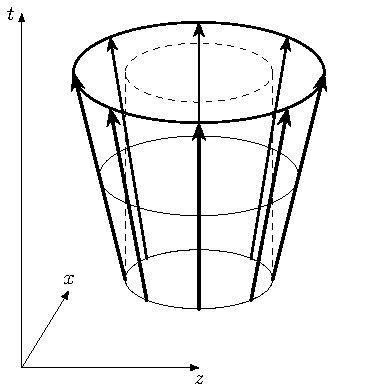
\includegraphics[width=.8\linewidth]{Figures/Expansion.pdf}
		\caption{A graphical representation of the expansion of a geodesic congruence.}
		\label{fig:exp}
	\end{minipage}\hfill
	\begin{minipage}[t]{.46\textwidth}
		\centering
		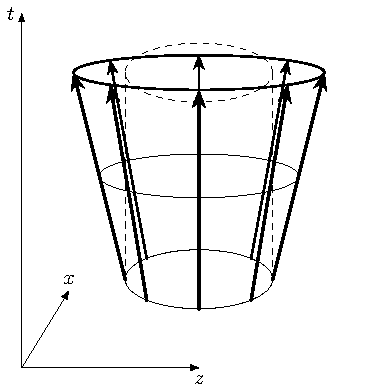
\includegraphics[width=.8\linewidth]{Figures/Shear.pdf}
		\caption{A graphical representation of the shear of a geodesic congruence.}
		\label{fig:shear}
	\end{minipage}
\end{figure}


We try to find the part of the metric $h_{\alpha\beta}$ that is transverse to our null vectors by supplementing the tangent field of that congruence with an auxiliary null field normalized against it. As noted above, our two null normals already satisfy $\ell_\mu k^\mu =-1$, so we may take $\ell_\mu$ as our auxiliary field of $k^\mu$ and vice versa. We then obtain an equation for the transverse metric as:

\begin{equation}
	h_{\alpha\beta} = g_{\alpha\beta} + k_\alpha \ell_\beta + \ell_\alpha k_\beta.
	\label{eq:transversemetric}
\end{equation}

This equation is symmetric under the exchange of $k$ and $\ell$, so both congruences share the same transverse metrics. We introduce the tensor fields

\begin{equation}
	B^{(k)}_{\alpha\beta} = k_{\alpha;\beta}\quad \text{and}\quad B^{(\ell)}_{\alpha\beta} = \ell_{\alpha;\beta}
\end{equation}
where the semicolon represents a covariant derivative with respect to the index after and immediately contract it with $h_{\alpha\beta}$ to create our objects of interest 

\begin{equation}
	\tilde{B}^{(k)}_{\alpha\beta} = h^\mu_{\hphantom{\mu}\alpha} h^\nu_{\hphantom{\nu}\beta}B^{(k)}_\mn \quad \text{and}\quad \tilde{B}^{(\ell)}_{\alpha\beta} = h^\mu_{\hphantom{\mu}\alpha} h^\nu_{\hphantom{\nu}\beta}B^{(\ell)}_\mn.
\end{equation}

\newpage
This allows us to more rigorously define our shear and expansion using this new tensor field $\tilde{B}_{\alpha\beta}$ and decomposing it

\begin{equation}
	\tilde{B}^{(v)}_\ab = \frac{1}{2}\theta^{(v)} h_\ab + \sigma^{(v)}_\ab + \omega^{(v)}_\ab
\end{equation}

Using $(v)$ to denote either $k$ or $\ell$. Here, $\theta^{(v)} = \tilde{B}^{(v)\hphantom{\alpha}\alpha}_{\hphantom{\alpha}\hphantom{\alpha}\alpha}$ or more explicitly $\theta^{(v)} = v^\alpha_{\hphantom{\alpha};\alpha}$ and $\sigma^{(v)}_\ab = \tilde{B}^{(v)}_{(\ab)} - \frac{1}{2}\theta^{(v)} h_\ab$, ignoring rotation $\omega^{(v)}_\ab$ and providing us with the equations relating the transverse metric to the shear and expansion.\newline

The expansion $\theta^{(\ell)}$ of the outward null normal $\ell$ is the core of our research, as we use this quantity to define a trapped surface using the change of the expansion:

\begin{equation}
	\dot{\theta}^{(\ell)} \leq 0
	\label{eq:trappedsurface}
\end{equation}

where the dot represents the derivative with respect to the time coordinate. To find our trapped surface or, in particular, marginally outer trapped surfaces, where equation \ref{eq:trappedsurface} becomes an equality, giving us the two conditions for MOTSs:

\begin{equation}
	\dot{\theta}^{(k)} < 0 \quad \text{and} \quad \dot{\theta}^{(\ell)} = 0.
\end{equation} 

We solve for these constraints this with a numerical Python script called MOTSfinder \cite{motsfinder}. \newline

The involvement of shear $\sigma^{(k)}$, in particular that of the inward null normal $k$ is a bit more subtle. We have found the equation $\sigma^{(k)}_\ab = \tilde{B}^{(k)}_{(\ab)} - \frac{1}{2}\theta^{(k)} h_\ab$ in the previous section. Using the basis of $k^\alpha$, $\ell^\alpha$, $\hat{e}^\alpha_{\hphantom{\alpha}A}$ and decomposing $B^{(k)}$ into a 2 x 2 matrix using that basis, we arrive $B^{(k)}_{AB} = B^{(k)}_\ab \hat{e}^\alpha_{\hphantom{\alpha}A}\hat{e}^\beta_{\hphantom{\beta}B}$. We will use this same method to create parameterizations for both the Riemann tensor and the Christoffel symbols, given as:

\begin{equation*}
	R_{AB} = R_{\alpha\mu\beta\nu} \hat{e}^\alpha_{\hphantom{\alpha}A}k^\mu\hat{e}^\beta_{\hphantom{\beta}B}k^\nu, \qquad \Gamma_{AB} = \hat{e}_{B\mu}\hat{e}^\mu_{\hphantom{\mu}A;\nu}k^\nu.
\end{equation*}

Where we have lost the index of $(v)$, since the same equations hold for both $k$ and $\ell$. We then decompose these into their irreducible parts:

\begin{equation*}
	B_{AB }= \frac{1}{2}\theta\delta_{AB} + \sigma_{AB} + \omega_{AB} \quad \text{and} \quad R_{AB} = \frac{1}{2}\mathscr{R} \delta_{AB}+ C_{AB}.
\end{equation*}

Where both $\sigma_{AB}$ and $C_{AB}$ are the symmetric and tracefree parts of their respective decompositions. Finally, we parametrize these matrices as 

\begin{equation*}
	\sigma_{AB} = 
	\begin{pmatrix}
		\sigma_+ & \sigma_\times \\
		\sigma_\times & -\sigma_+ 
	\end{pmatrix}
	\quad \text{and} \quad
	C_{AB}
	\begin{pmatrix}
		C_+ & C_\times \\
		C_\times & -C_+ 
	\end{pmatrix}.
\end{equation*}

for both $\sigma_{AB}$ and $C_{AB}$.
\newpage

For the matrices $\omega_{AB}$ and $\Gamma_{AB}$, we use

\begin{equation*}
	\omega_{AB} = 
	\begin{pmatrix}
		0 & \omega \\
		-\omega & 0 
	\end{pmatrix}
	\quad \text{and} \quad
	\Gamma_{AB}
	\begin{pmatrix}
		0 & \Gamma \\
		-\Gamma & 0 
	\end{pmatrix}.
\end{equation*}

Applying these to the main evolution equation for $B_{AB}$, where

\begin{equation*}
	\frac{dB_{AB}}{d\lambda} = -B_{AC}B^C_{\hphantom{C}B} - R_{AB} + \Gamma_A^{\hphantom{A}C}B_{CB}+\Gamma_B^{\hphantom{B}C}B_{AC},
\end{equation*}

we arrive at our final set of evolution equations:

\begin{equation}
	\begin{cases}
		\frac{d\theta}{d\lambda} = -\frac{1}{2}\theta^2 - 2(\sigma_+^2 + \sigma_\times^2) + 2\omega^2 - \mathscr{R} \\
		\frac{d\sigma_+}{d\lambda} = -\theta\sigma_+ - C_+ + 2\Gamma\sigma_\times\\
		\frac{d\sigma_\times}{d\lambda} = -\theta\sigma_\times - C_\times - 2\Gamma\sigma_+\\
		\frac{d\omega}{d\lambda} = -\theta\omega\\
	\end{cases}
	\label{eq:evolutioneqs}
\end{equation}

In particular, the second and third equations are the most interesting, as it seems that the evolution of both shears is directly related to the Weyl tensor. As we know, the Weyl tensor relates to the amount of gravitational radiation in our spacetime. So curiously, the evolution of the shear tells us something about gravitational radiation! \newline 

To further simplify these equations, we can take $\hat{e}^\alpha_{\hphantom{\alpha}A}$ to be parallel transported along the congruence, making $\Gamma_{AB}$ vanish and leaving us with the equations without the cross-terms as

\begin{equation}
	\begin{cases}
		\frac{d\sigma_+}{d\lambda} = -\theta\sigma_+ - C_+, \\
		\frac{d\sigma_\times}{d\lambda} = -\theta\sigma_\times - C_\times .
	\end{cases}
	\label{eq:shearevolution}
\end{equation} 


\section{ADM-formalism}

While in general relativity we usually treat spacetime as a four-dimensional volume, with time 'just' being one of these four dimensions, we would still like to be able to look at the time evolution of certain quantities. We therefore want to decompose our 4-dimensional spacetime as the time evolution of 3-dimensional hypersurfaces. A way of doing this without losing the abilities of general relativity, was first introduced by Arnowitt, Deser and Misner. This formalism is therefore called the ADM-formalism or the Hamiltonian formulation of general relativity. We will follow a review by A. Corichi and D. Núñez \cite{introductiontoadm}.\newline

Central to this formalism are three different properties: the lapse $N$, the shift vector $N^i$ and the induced metric $\gamma_{ij}$. Think of this formalism as breaking down our spacetime into these 'slices'. The lapse tells us how far apart those slices are from each other, the shift where the same point goes between two slices, and the induced metric shows us the curvature of each three-dimensional hypersurface.

\begin{figure}[!htb]
	\centering
	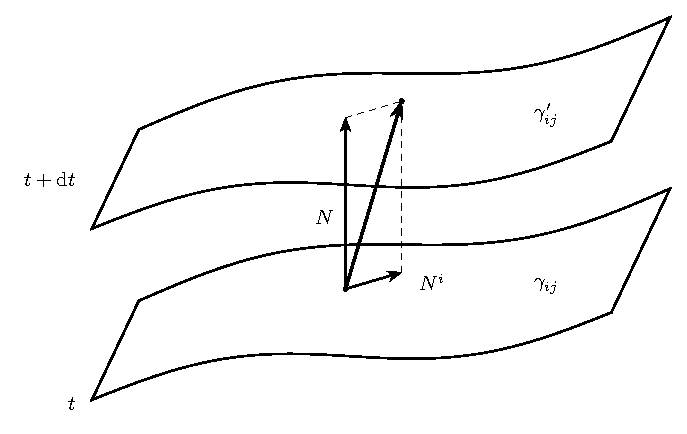
\includegraphics[width=0.8\textwidth]{Figures/ADM_slices.pdf}
	\caption{An example of the ADM-slicing of a spacetime into hypersurfaces, inspired by Corichi and Núñez \cite{introductiontoadm}.}
	\label{fig:admslicing}
\end{figure}

Figure \ref{fig:admslicing} shows us, hopefully more intuitively, what the slicing of a spacetime looks like. We can therefore study just these hypersurfaces and look at their evolution: we can look at general relativity as a dynamical theory. The time coordinate here can then be regarded as the slicing of the spacetime, doing away with a more traditional notion of time. The four-dimensional metric in this formalism is then written in the following form:

\begin{equation}
	ds^2 = (N^aN_a-N^2)dt^2 +2N_adx^adt+\gamma_{ab}dx^adx^b.
	\label{eq:admmetric}
\end{equation}


The method for changing four-dimensional metrics into the ADM-form is then actually quite easy. We will look at a general example using an arbitrary metric:

\begin{equation}
	g = 
	\begin{pmatrix}
		g_{tt} & g_{tx} & g_{ty} & g_{tz} \\
		g_{xt} & g_{xx} & g_{xy} & g_{xz} \\
		g_{yt} & g_{yx} & g_{yy} & g_{yz} \\
		g_{zt} & g_{zx} & g_{zy} & g_{zz} 
	\end{pmatrix}.
\end{equation}

We equate the purely temporal part in equation \ref{eq:admmetric} to $g_{tt}$, take the purely spatial induced metric to be the lower 3 x 3 matrix, and use the mixed part of the equation to our leftover six entries, resulting in the following set of equations:

\begin{equation}
	(N^aN_a-N^2) = g_{tt}, \qquad N_adx^a = g_{ta}dx^a \quad \text{and} \quad \gamma_{ij} = 
	\begin{pmatrix}
		g_{xx} & g_{xy} & g_{xz} \\
		g_{yx} & g_{yy} & g_{yz} \\
		g_{zx} & g_{zy} & g_{zz} 
	\end{pmatrix}.
\end{equation}

Usually, we will solve the second and third equations first to find our shift vector and induced metric, then solve the first to find our lapse.

\subsection{Extrinsic curvature}

Another reason this formalism works for our research is due to the nice expression for the extrinsic curvature in the ADM formalism. The extrinsic curvature is required for the numerical program to work, so let us look at what it actually means. The extrinsic curvature $K_\mn$ is given by:

\begin{equation}
	K_{ij} = \frac{1}{N}(D_i N_j + D_j N_i - \partial_t\gamma_{ij})
	\label{eq:extrinsiccurvature}
\end{equation}

Where, as you can see, all of our ADM variables show up. $K_\mn$ is different from intrinsic curvature, often described as the curvature you can 'feel' if you would be standing on such a surface. Extrinsic curvature would not be felt by somebody living on a extrinsically curved surface.\newline

Using this, we will define something called the conjugate momentum $\pi^{ij}$ as follows:

\begin{equation}
	\pi^{ij} = -\sqrt{\gamma}(K^{ij} - \gamma^{ij}K)
\end{equation}

Where $\gamma$ is the determinant of the induced metric and $K = \gamma^{ij}K_{ij}$ is the trace of the extrinsic curvature.

\section{The Kerr-Schild form of metrics}

Another useful mathematical tool for our calculations will be the Kerr-Schild form of a specific class of spacetimes, as derived by its Kerr and Schild \cite{Kerr2009-nk} as:

\begin{equation}
	g_\mn = (\eta_\mn + 2Hk_\mu k_\nu)dx^\mu dx^\nu.
	\label{eq:ksform}
\end{equation}

Where $\eta_\ab$ is the Minkowski flat spacetime, and our total spacetime is just that with a pertubation by some null vectors $k_\alpha$ and a scalar function $H$. This metric has some nice properties, most notably that it is asymptotically flat depending on the form of $H$, recovering our Minkowski metric in the limit as $r  \rightarrow \infty$. Casting, for example, the Schwarzschild metric into this form, we obtain:

\begin{equation}
	ds^2 = -dt^2 dx^2 + dy^2 + dz^2 +\frac{2M}{r}(dt+dr)^2.
\end{equation}

As we can see, as $r$ approaches infinity, we get our flat spacetime back, as you would expect. This recasting into the Kerr-Schild form makes this property of the Schwarzschild metric more explicit, being valuable in our research.


\section{Suppressing dimensions}

This study will look at axisymmetric spacetimes only, so we can do away with one of our traditional axes for the sake of clarity. We can then plot the time evolution of MOTSs on a 3-dimensional space. Taking the time coordinate to be the vertical, we will only plot the x-z plane. \newline

As an example, the Schwarzschild spacetime is usually depicted as a sphere. Suppressing one dimension will then turn this into a circle. Plotting its time evolution, we obtain a figure as such:

\begin{figure}[!htb]
	\centering
	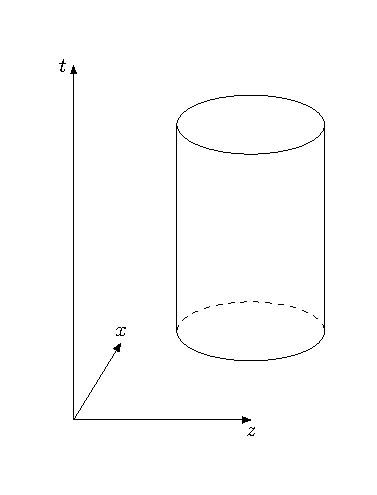
\includegraphics[width=0.5\textwidth]{Figures/reference.pdf}
	\caption{The time evolution of a MOTS in the Schwarzschild spacetime.}
	\label{fig:reference}
\end{figure}

We will use figures like \ref{fig:reference} often, to show what is actually happening with different slicings and what we can expect to see in the x-z plane for these slicings.

\section{Using MOTSfinder}

MOTSfinder is, as the name suggests, a numerical algorithm to find MOTSs, restricted to axisymmetric cases. This program has been written by D. Pook-Kolb, O. Birnholtz, B. Krishnan and E. Schnetter in 2019 \cite{motsfinder} and is readily documented on Pook-Kolb's GitHub, which has been extremely useful in this study. This section will explain how we used this program to find our MOTSs.\newline


\subsection{Mathematica}
Firstly, we need to implement a new analytical metric for each slicing. This requires the ADM-variables of the induced metric, shift vector, lapse, and extrinsic curvature, as discussed in a previous section. As this becomes quite cumbersome to calculate by hand, we defer to Wolfram Mathematica \cite{Mathematica} using the Riemannian Geometry \& Tensor Calculus (RGTC) \cite{RGTCref} and Exterior Differential Calculus (EDC) packages, both created by S. Bonanos. These combine into a single package, called EDCRGTC.\newline

Here we used the Kerr-Schild form of our metrics of interest and used the tools of EDCRGTC to compute the lapse, shift vector and extrinsic curvature. To then check the validity of our calculations, we used two constraints:

\begin{equation}
	R + K^2 - K_{ij}K^{ij} = G_{tt} \quad \text{and} \quad \nabla_j \pi^{ij} = 0.
\end{equation}

The first one is called the Hamiltonian constraint, with the Ricci scalar being that of the induced metric $\gamma_{ij}$. For vacuum spacetimes, we know that $G_{tt}=0$, which is quite useful. The other is the momentum constraint, which is only zero in a vacuum. For the Schwarzschild and Minkowski spacetimes, these are actually quite quick and easy to calculate. For the sliced Vaidya spacetime, we started to run into runtime limits, so we were only able to check the Hamiltonian constraint for this spacetime. As our methods proved to work, we can be confident enough to keep going.

\subsection{MOTSfinder}

Now that we have analytical expressions for our metrics, we can switch over to the numerical part of these calculations and implement a new class of the form \verb*|motsfinder.metric.analytical.metricX|. We implement the values we found in our Mathematica phase, then use the \verb*|find_AH| command to find our MOTSs. The actual code used to obtain these results is linked in Appendix \ref{chapter:rdm}.\newline

After finding our MOTSs, we want to look at its geometrical properties. To see what happens along the boundary, we use the \verb*|spinsfast| Python package to expand the shear and expansion of these MOTSs into spherical harmonics, plotting the shear and expansion of both the ingoing and outgoing null normals. Of course, by definition, the expansion of the outgoing null normal is zero along a MOTS, so we usually disregard that plot. Finally, we can analyze the time evolution of the spin-weighted spherical harmonics to better understand the gauge properties of different slicings.

\chapter{Finding MOTS: examples}

Now that we have thoroughly discussed the background of why this works, we have figured out a step-by-step way to find the MOTSs of any spacetime as follows:

\begin{enumerate}
	\item Transform our metric to its Kerr-Schild form.
	\item Find all ADM-variables of this metric using Mathematica.
	\item Check these variables using the Hamiltonian and momentum constraints.
	\item Transfer these properties to the appropriate class within MOTSfinder.
	\item Find our MOTSs using \verb*|find_AH|.
	\item Expand these into spherical harmonics with \verb*|spinsfast|.
	\item Analyse!
\end{enumerate}

This seems simple enough, so let us go through some examples, starting with the simplest: the Minkowski spacetime.

\section{The Minkowski spacetimes}

\subsection{Definitions and slicing}

As we all know, the Minkowski spacetime is given as:

\begin{equation}
	ds^2 = -dt^2 + dx^2 + dy^2 + dz^2
\end{equation}

This metric is already in Kerr-Schild form, with $H = 0$. Therefore we can continue by rewriting this to the ADM-form using our equations

\begin{equation}
	(N^aN_a-N^2) = g_{tt}, \qquad N_adx^a = g_{ta}dx^a \quad \text{and} \quad \gamma_{ij} = 
	\begin{pmatrix}
		g_{xx} & g_{xy} & g_{xz} \\
		g_{yx} & g_{yy} & g_{yz} \\
		g_{zx} & g_{zy} & g_{zz} 
	\end{pmatrix}.
\end{equation}

We get, in this case, the following:

\begin{equation}
	(N^aN_a-N^2) = -1, \qquad N_adx^a = 0 \quad \text{and} \quad \gamma_{ij} = 
	\begin{pmatrix}
		1 & 0 & 0 \\
		0 & 1 & 0 \\
		0 & 0 & 1 
	\end{pmatrix}.
\end{equation}

So our induced metric is just the identity in three dimensions. Our shift vector is zero, which means that $N^2 = 1$. Since our shift vector is zero, our extrinsic curvature $K_{ij}$ is also zero in this slicing.

\subsection{New slicing}

Now we will change the slicing of our spacetime, defining a new time coordinate $\tilde{t} = t + f(z)$, where $f(z)$ is an arbitrary function only dependent on our $z$-coordinate. Rewriting $dt$ into $d\tilde{t} - f'dz$ gives us the following four-metric:
\begin{equation}
	\begin{pmatrix}
		-1 & 0 & 0 & f'\\
		0 & 1& 0 & 0\\
		0 & 0 & 1 & 0\\
		f'& 0 & 0 & 1-f'^2
	\end{pmatrix}
\end{equation}

Now our induced metric and shift transforms into
\begin{equation}
	N_a =
	\begin{pmatrix}
		0 \\
		0\\
		f'
	\end{pmatrix}
	 \quad \text{and} \quad \gamma_{ij} = 
	\begin{pmatrix}
		1 & 0 & 0 \\
		0 & 1 & 0 \\
		0 & 0 & 1 
	\end{pmatrix}.
\end{equation}

Our equation for the lapse then becomes:

\begin{equation}
	  N^2 = 1 + N^aN_a.
\end{equation}

We know that $N^a = \gamma^{a\lambda}N_\lambda$, so we get $N^2 = \frac{1}{1-f'^2}$. With these calculated, we will arrive at our extrinsic curvature $K_{ij}$

\begin{equation}
	K_{ij} =
	\begin{pmatrix}
		0& 0 & 0 \\
		0 & 0 & 0 \\
		0 & 0 & -\sqrt{\frac{1}{1-f'^2}}f'' 
	\end{pmatrix}.
\end{equation}

\newpage

\subsection{Discussion of the results}

As we have shown, changing the slicing of our spacetime creates a nonzero extrinsic curvature. However, this is still not a black hole spacetime, so there is no MOTS. We can show this as such:

\begin{equation*}
	\dot{\theta} = \partial_{\tilde{t}} K^i_{\hphantom{i}i},
\end{equation*} 

\begin{equation*}
	\dot{\theta} = \partial_{\tilde{t}}\frac{\sqrt{\frac{1}{1-f'^2}}f''}{(f'-1)(f'+1)}.
\end{equation*}
So $\dot{\theta} = 0$ holds everywhere. There are no MOTSs anywhere, as we would expect.
\section{The Schwarzschild spacetimes}
\subsection{Definitions and slicing}

We use Kerr-Schild coordinates for the Schwarzschild metric:

\begin{equation}
    ds^2 = -dt^2 + dx^2+dy^2+dz^2+\frac{2M}{r}(dt+dr)^2.
\end{equation}

These need to be cast into the ADM-form. Writing out the quadratic term gives us:

\begin{equation}
    ds^2 = -dt^2 + dx^2+dy^2+dz^2+\frac{2M}{r}(dt^2+2dtdr+dr^2),
\end{equation}
\begin{equation}
    ds^2 = \left(\frac{2M}{r}-1\right)dt^2 + dx^2+dy^2+dz^2+\frac{2M}{r}dr^2 + \frac{2M}{r}2dtdr.
\end{equation}

Since $dr = \frac{x}{r}dx+\frac{y}{r}dy+\frac{z}{r}dz$, or $\frac{x_i}{r}dx^i$. This gives us $dr^2 = \frac{x_ix_j}{r^2}dx^idx^j$. Implementing this in our equation gives us:

\begin{equation}
     ds^2 = \left(\frac{2M}{r}-1\right)dt^2 + dx^2+dy^2+dz^2+\frac{2M}{r}\frac{x_ix_j}{r^2}dx^idx^j + \frac{2M}{r}\frac{2x_i}{r}dx^idt,
\end{equation}

\begin{equation}
    ds^2 = \left(\frac{2M}{r}-1\right)dt^2 + \frac{2M}{r}\frac{2x_i}{r}dx^idt +\left(\frac{2M}{r}\frac{x_ix_j}{r^2}+\delta_{ij}\right)dx^idx^j .
\end{equation}

Now comparing this to our general ADM form, we get the following set of equations:


\begin{equation}
    \begin{cases}
        \left(\frac{2M}{r}-1\right)dt^2= (N^aN_a-N^2)dt^2\\
        \frac{2M}{r}\frac{2x_i}{r}dx^idt = 2N_idx^idt\\
        \left(\frac{2M}{r}\frac{x_ix_j}{r^2}+\delta_{ij}\right)dx^idx^j = \gamma_{ij}dx^idx^j\\
    \end{cases}\,
\end{equation}

Therefore our induced metric $\gamma_{ij}$ is given by $ \left(\frac{2M}{r}\frac{x_ix_j}{r^2}+\delta_{ij}\right)$, or, in matrix form:

\begin{equation}
	\gamma_{ij}=
	\begin{pmatrix}
		\frac{2M}{r}\frac{x^2}{r^2}+1 & \frac{2M}{r}\frac{xy}{r^2} & \frac{2M}{r}\frac{xz}{r^2}\\
		\frac{2M}{r}\frac{xy}{r^2} & \frac{2M}{r}\frac{y^2}{r^2}+1 & \frac{2M}{r}\frac{yz}{r^2}\\
		\frac{2M}{r}\frac{xz}{r^2} & \frac{2M}{r}\frac{yz}{r^2} & \frac{2M}{r}\frac{z^2}{r^2}+1
	\end{pmatrix}.
\end{equation}


The second equation gives the shift vector $N_i$:
\begin{equation}
    \frac{2M}{r}\frac{2x_i}{r}dx^idt = 2N_adx^adt\\,
\end{equation}

\begin{equation}
    N_i = \frac{2M}{r}\frac{x_i}{r}.
\end{equation}

Finally, the lapse is given by the first equation:
\begin{equation}
    \left(\frac{2M}{r}-1\right)dt^2= (N^aN_a-N^2)dt^2.
\end{equation}

$N_aN^a$ equals $N_a \gamma^a_{\hphantom{a}\lambda}N^\lambda$, with $\gamma^a_{\hphantom{a}\lambda}N^\lambda = \frac{2M}{r+2M}x^a$. Therefore $N_aN^a = \frac{4M^2}{r(r+2M)}$. Casting this into our first equation gives us:

\begin{equation}
    N^2= \frac{4M^2}{r(r+2M)}-\frac{2M}{r}+1\\ ,
\end{equation}

\begin{equation}
    N= \sqrt{\frac{r}{r+2M}}.
\end{equation}

\subsection{New slicing}

Now we will again change the slicing of our spacetime, defining a new time coordinate $\tilde{t} = t + f(z)$, where $f(z)$ is an arbitrary function only dependent on our $z$-coordinate. Rewriting $dt$ into $d\tilde{t} - f'dz$ gives us the following four-metric:

\begin{equation*}
	\begin{pmatrix}
	    \frac{2M}{r}-1 & \frac{2M}{r}\frac{x}{r} & \frac{2M}{r}\frac{y}{r} & \frac{2M}{r}\left(\frac{z}{r}+\frac{f'}{r}\right)-f'\\
	    \frac{2M}{r}\frac{x}{r} & 1+\frac{2M}{r}\frac{x^2}{r^2} & \frac{2M}{r}\frac{xy}{r^2} &\frac{2M}{r}\left(\frac{xz}{r^2}+\frac{xf'}{r^2}\right)\\
	    \frac{2M}{r}\frac{y}{r} & \frac{2M}{r}\frac{xy}{r^2} & 1+\frac{2M}{r}\frac{y^2}{r^2} &\frac{2M}{r}\left(\frac{xy}{r^2}+\frac{yf'}{r^2}\right)\\
	    \frac{2M}{r}\left(\frac{z}{r}+\frac{f'}{r}\right)-f' & \frac{2M}{r}\left(\frac{xz}{r^2}+\frac{xf'}{r^2}\right) & \frac{2M}{r}\left(\frac{yz}{r^2}+\frac{yf'}{r^2}\right)  & 1 - f'^2 + \frac{2M}{r}\left(\frac{z^2}{r^2}+\frac{2zf'}{r}+f'^2\right)
	\end{pmatrix}.
\end{equation*}
This gives us the following values for the induced metric:
\begin{equation}
	\gamma_{ij}=
	\begin{pmatrix}
	     1+\frac{2M}{r}\frac{x^2}{r^2} & \frac{2M}{r}\frac{xy}{r^2} &\frac{2M}{r}\left(\frac{xz}{r^2}+\frac{xf'}{r^2}\right)\\
	     \frac{2M}{r}\frac{xy}{r^2} & 1+\frac{2M}{r}\frac{y^2}{r^2} &\frac{2M}{r}\left(\frac{xy}{r^2}+\frac{yf'}{r^2}\right)\\
	     \frac{2M}{r}\left(\frac{xz}{r^2}+\frac{xf'}{r^2}\right) & \frac{2M}{r}\left(\frac{yz}{r^2}+\frac{yf'}{r^2}\right)  & 1 - f'^2 + \frac{2M}{r}\left(\frac{z^2}{r^2}+\frac{2zf'}{r}+f'^2\right)
	\end{pmatrix}.
\end{equation}
The following values for the shift vector:

\begin{equation}
	N_i = 
    \frac{2M}{r}\begin{pmatrix}
     \frac{x}{r} \\ 
     \frac{y}{r} \\ 
     \frac{z}{r}+\frac{f'}{r}-\frac{r}{2M}f'
\end{pmatrix}.
\end{equation}

And the lapse:

\begin{equation}
    N^2 = \frac{r^3}{r^2(2M+r)+4Mrzf'-(r^3+2Mz^2)f'^2}.
\end{equation}

Now, this is for the general case of $\tilde{t} = t + f(z)$. We now need to define our slicing function $f(z)$. Following the example set by Schnetter and Krishnan \cite{badripaper}, we pick $f(z) = -\alpha z$. A nice property of this slicing function is that it allows us to return to our 'normal' slicing by setting $\alpha$ equal to zero. This allows us to only have to implement one metric into the MOTSfinder codebase, that of the new slicing.

\subsection{MOTSs}

After implementing these calculations into MOTSfinder, we find following MOTSs for different values of $\alpha$:

\begin{figure}[!htb]
	\centering
	\begin{minipage}[t]{.46\textwidth}
		\centering
		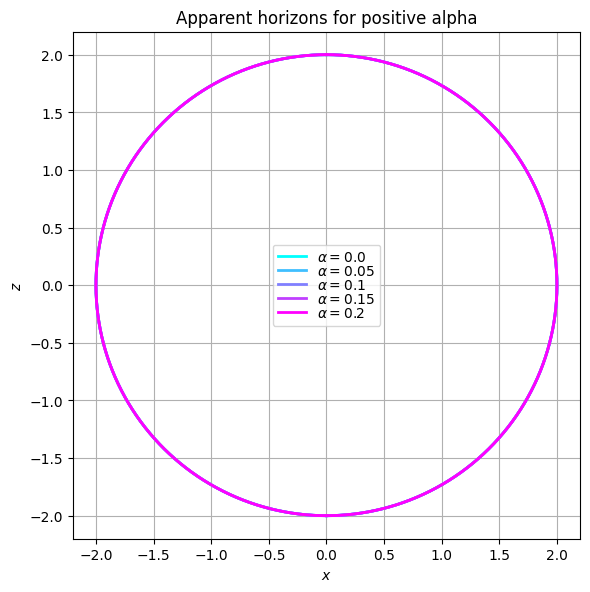
\includegraphics[width=.8\linewidth]{Figures/MOTS/AHposAlphaSchwarzschild.png}
		\caption{Apparent horizons found for a time coordinate defined by a slicing with a positive $\alpha$}
		\label{fig:schwarzschildmotspositivealpha}
	\end{minipage}\hfill
	\begin{minipage}[t]{.46\textwidth}
		\centering
		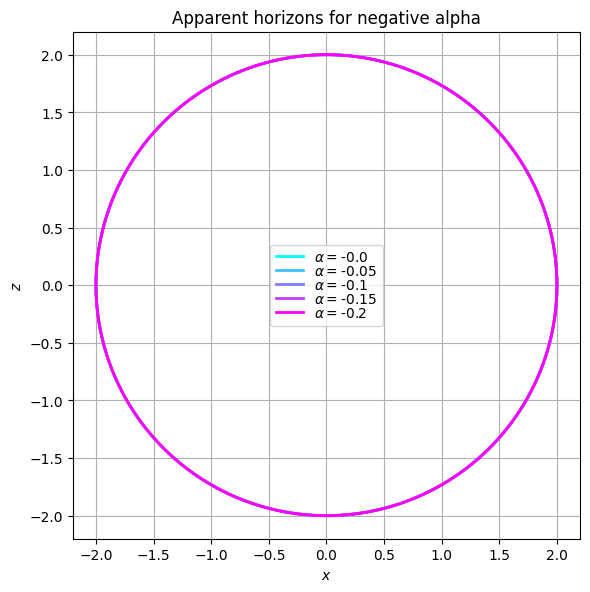
\includegraphics[width=.8\linewidth]{Figures/MOTS/AHnegAlphaSchwarzschild.png}
		\caption{Apparent horizons found for a time coordinate defined by a slicing with a negative $\alpha$}
		\label{fig:schwarzschildmotsnegativealpha}
	\end{minipage}
\end{figure}
As we can see in figures \ref{fig:schwarzschildmotspositivealpha} and \ref{fig:schwarzschildmotsnegativealpha}, these MOTSs do not change for different slicings. The MOTSs all lie on top of each other, so we only see the MOTS for $\alpha = \pm 0.2$.

\newpage
\subsection{Discussion of the results}

As we can see in figures \ref{fig:schwarzschildmotspositivealpha} and \ref{fig:schwarzschildmotsnegativealpha}, the MOTSs do not change for different values of $\alpha$. A very intuitive way to look at this is to refer back to figure \ref{fig:reference}, and see what these different slicings actually look like in that picture. We then will find the following:

\begin{figure}[!htb]
	\centering
	\begin{minipage}[t]{.46\textwidth}
		\vspace{0pt}
		\centering
		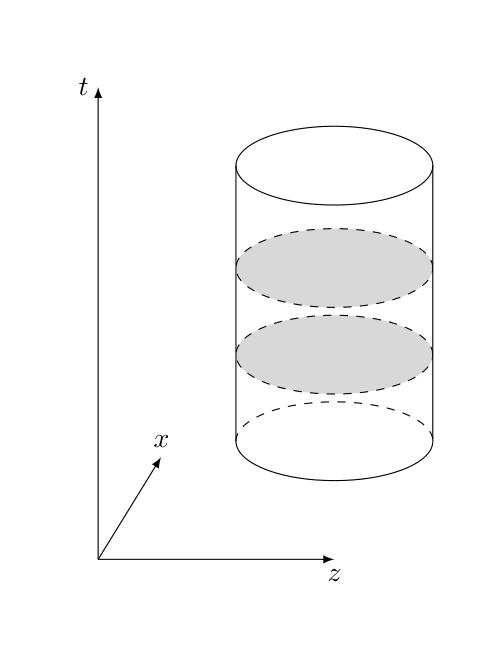
\includegraphics[height=6cm]{Figures/normal_sliced_schwarzschild-1.png}
		\caption{The time evolution of the Schwarzschild black hole slicing for $\alpha = 0$}
		\label{fig:refnormalslicingschwarzschild}
	\end{minipage}\hfill
	\begin{minipage}[t]{.46\textwidth}
		\vspace{0pt}
		\centering
		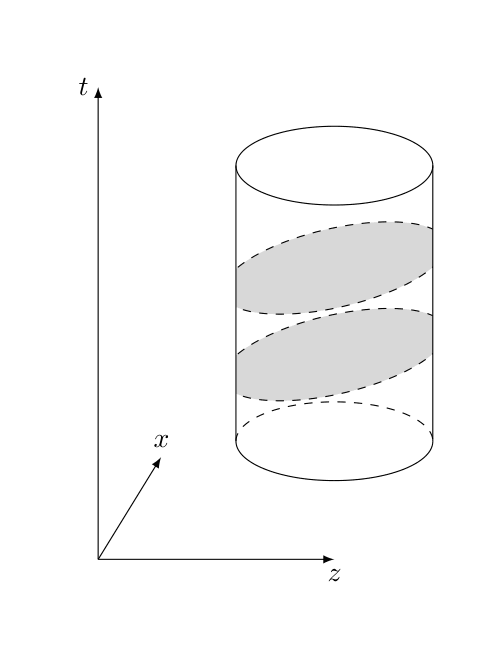
\includegraphics[height=6cm]{Figures/funky_schwarzschild-1.png}
		\caption{The time evolution of the Schwarzschild black hole slicing for a nonzero $\alpha$}
		\label{fig:reffunkyslicingschwarzschild}
	\end{minipage}
\end{figure}

These figures, when projected unto the x-z plane, produce the figures you can see in the previous section. This gives us confidence that we can trust MOTSfinder to find the correct MOTSs, and also that we have a solid grasp on our expectations of the shape of different MOTSs. This interpretation makes sense to us when we realize that the MOTS for a Schwarzschild spacetime is actually equal to the event horizon. The event horizon should be slicing-invariant, so the MOTSs are too. Now, we will start to look at a slightly more difficult example, that of a Vaidya black hole. 

\section{The Vaidya spacetimes}
\subsection{Definitions and slicing}

We use the ingoing Vaidya metric in Eddington-Finkelstein coordinates, given by \cite{VAIDYASPACETIME}:

\begin{equation}
	ds^2  	= -\left(1-\frac{2M(v)}{r}\right) dv^2 +2dvdr+r^2d\theta^2 + r^2\sin^2\theta d\phi^2 .
\end{equation}

We use the ingoing metric, as we want to look at a black hole absorbing null radiation.\newline

As usual, we transform this into Kerr-Schild coordinates, resulting in

\begin{equation}
	ds^2 = -dt^2 + dx^2+dy^2+dz^2+\frac{2M(t+r)}{r}(dt+dr)^2,
	\label{eq:vaidyametrickerrschild}
\end{equation}

where we transformed the usual Vaidya null coordinate $v$ to $t+r$. The derivation follows the same as the derivation for the Schwarzschild metric in Kerr-Schild coordinates.

\subsection{New slicing}

We use the same slicing as the case for the Schwarzschild metric, where $\tilde{t} = t + f(z)$. This results in the following metric:

\begin{equation}
	g_\mn = 
	\begin{pmatrix}
		\frac{2M(\tilde{t}-r)}{r} - 1 & \frac{2M(\tilde{t}-r)}{r}\frac{x}{r} & \frac{2M(\tilde{t}-r)}{r}\frac{y}{r} &
		\frac{2M(\tilde{t}-r)}{r^2} \left(\frac{z+f'(z)}{r}\right) - f'(z)\\
		\frac{2M(\tilde{t}-r)}{r}\frac{x}{r}  & \frac{2M(\tilde{t}-r)}{r}\frac{x^2}{r^2}  - 1 & \frac{2M(\tilde{t}-r)}{r}\frac{xy}{r^2} &
		\frac{2M(\tilde{t}-r)}{r^2}\frac{x}{r} \left(\frac{z+f'(z)}{r}\right)\\
		\frac{2M(\tilde{t}-r)}{r}\frac{y}{r}  & \frac{2M(\tilde{t}-r)}{r}\frac{xy}{r^2}  - 1 & \frac{2M(\tilde{t}-r)}{r}\frac{y^2}{r^2} &
		\frac{2M(\tilde{t}-r)}{r^2}\frac{y}{r} \left(\frac{z+f'(z)}{r}\right)\\
		\left(\frac{z+f'(z)}{r}\right) - f'(z)&
		\frac{2M(\tilde{t}-r)}{r^2}\frac{x}{r} \left(\frac{z+f'(z)}{r}\right) &
		\frac{2M(\tilde{t}-r)}{r^2}\frac{y}{r} \left(\frac{z+f'(z)}{r}\right) &
		1 - f'(z)^2 + \frac{2M(\tilde{t}-r)}{r^2} \left(\frac{z+f'(z)}{r}\right)\\
		
	\end{pmatrix}.
\end{equation}

This gives the following induced metric $\gamma_{ij}$


\begin{equation}
	\gamma_{ij}=
	\begin{pmatrix}
		 \frac{2M(\tilde{t}-r)}{r}\frac{x^2}{r^2}  - 1 & \frac{2M(\tilde{t}-r)}{r}\frac{xy}{r^2} &
		\frac{2M(\tilde{t}-r)}{r^2}\frac{x}{r} \left(\frac{z+f'(z)}{r}\right)\\
		 \frac{2M(\tilde{t}-r)}{r}\frac{xy}{r^2}  - 1 & \frac{2M(\tilde{t}-r)}{r}\frac{y^2}{r^2} &
		\frac{2M(\tilde{t}-r)}{r^2}\frac{y}{r} \left(\frac{z+f'(z)}{r}\right)\\
		\frac{2M(\tilde{t}-r)}{r^2}\frac{x}{r} \left(\frac{z+f'(z)}{r}\right) &
		\frac{2M(\tilde{t}-r)}{r^2}\frac{y}{r} \left(\frac{z+f'(z)}{r}\right) &
		1 - f'(z)^2 + \frac{2M(\tilde{t}-r)}{r^2} \left(\frac{z+f'(z)}{r}\right)\\
		
	\end{pmatrix},
\end{equation}

shift vector $N_i$ and lapse $N$
\begin{equation}
	N_i = 
	\begin{pmatrix}
		\frac{2M(\tilde{t}-r)}{r}\frac{x}{r} \\ \frac{2M(\tilde{t}-r)}{r}\frac{y}{r}\\
		\frac{2M(\tilde{t}-r)}{r^2} \left(\frac{z+f'(z)}{r}\right) - f'(z)\\
	\end{pmatrix}
	\quad \text{and} \quad
	N^2 = \frac{r^2}{-r^2(f'(z)-1)+\frac{2M(\tilde{t}-r)}{r}\left(r+2rzf'(z)+z^2f'(z)^2\right)}.
\end{equation}


\subsection{MOTSs}
For finding the MOTSs, we will again have to define a slicing function and we will use the same function $f(z) = -\alpha z$ as in the Schwarzschild case. Furthermore, we have to look at an appropriate mass function $M(\tilde{v})$. We again follow our guiding paper \cite{badripaper} and choose

\begin{equation}
	M(\tilde{v}) = 
	\begin{cases}
		0 &\text{for} \ \tilde{v} \leq 0 \\
		M_0 \frac{\tilde{v}^2}{\tilde{v}^2+W^2} & \text{for} \ \tilde{v} > 0 \\
	\end{cases}
	\label{eq:massfunc}
\end{equation}

where $W$ is a variable we can fine-tune, choosing the 'steepness' of the slope of the mass function, and $\tilde{v} = \tilde{t} - r$ our sliced Vaidya time. 

\newpage

\begin{figure}[!htb]
	\centering
	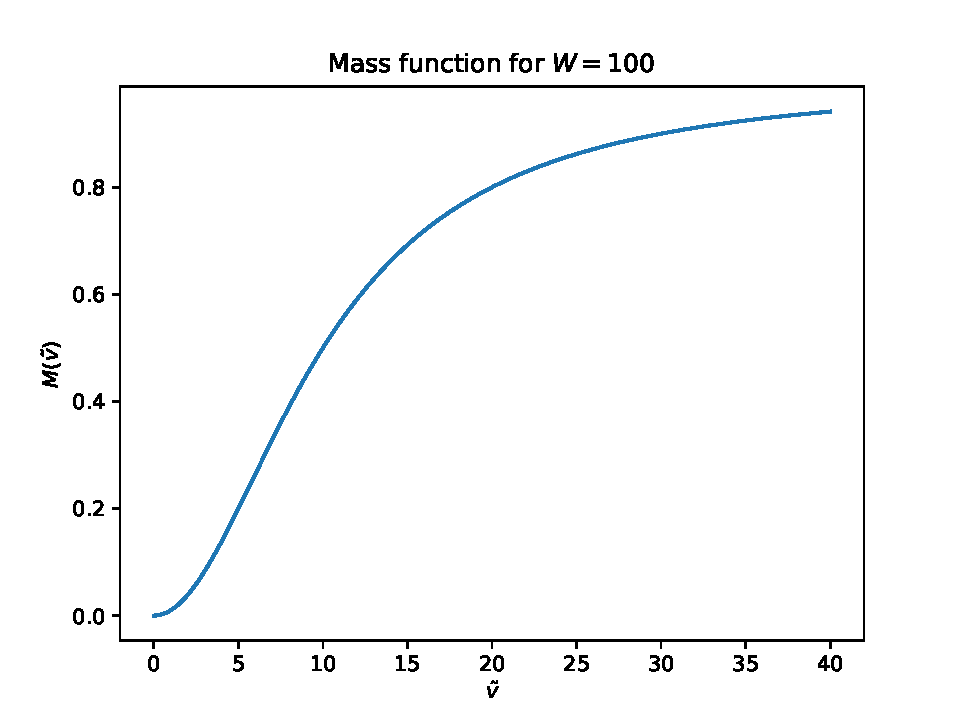
\includegraphics[width=0.5\textwidth]{Figures/massfuncw100.pdf}
	\caption{Our chosen mass function (see equation \ref{eq:massfunc}, with parameters $W = 100$ and $M_0 = 1$), gradually increasing from zero to our $M_0$.}
	\label{fig:massfunc}
\end{figure}

We will choose $W = 100$ for our normally sliced Vaidya black hole and $W = 1/10$ for our new slicing. We do this to clearly be able to see the effect of the different slicings. Picking $M_0 = 1$, this function is shown in figure \ref{fig:massfunc}. Using a slicing variable of $\alpha = \frac{10}{11}$, we can finally find our MOTSs.

\begin{figure}[!htb]
	\centering
	\begin{minipage}[t]{.47\textwidth}
		\centering
		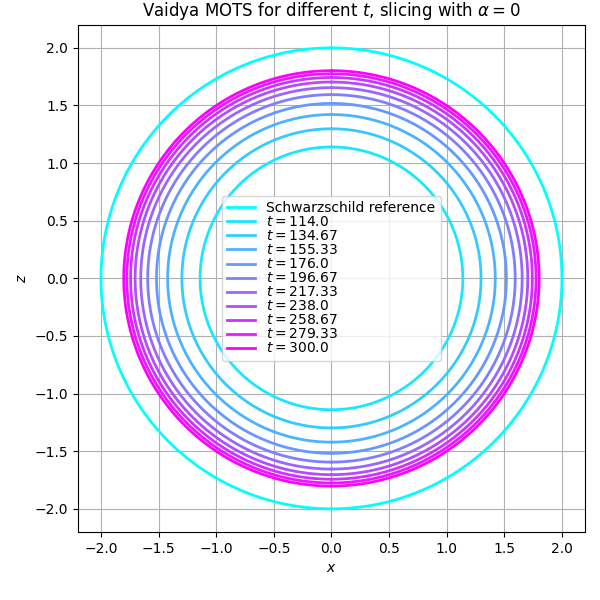
\includegraphics[width=\linewidth]{Figures/MOTS/vaidyamotspresentation.png}
		\caption{The time evolution of the Vaidya black hole slicing for an $\alpha = 0$.}
		\label{fig:vaidyamots}
	\end{minipage}\hfill
	\begin{minipage}[t]{.47\textwidth}
		\centering
		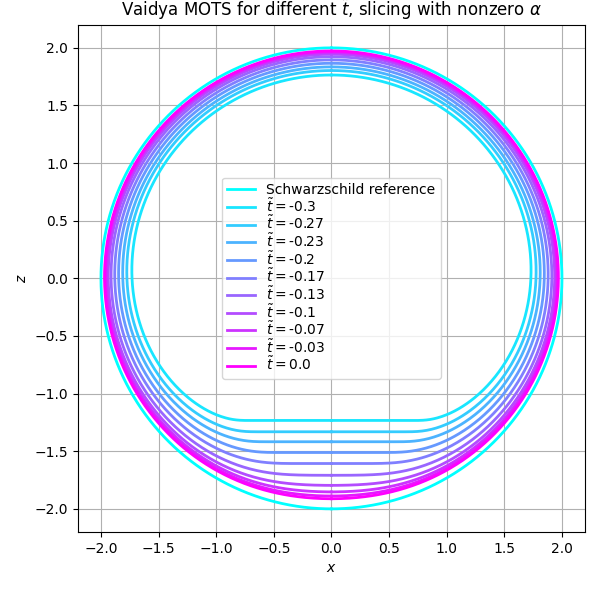
\includegraphics[width=\linewidth]{Figures/MOTS/vaidyamotspresentationsliced.png}
		\caption{The time evolution of the Vaidya black hole slicing for $\alpha = \frac{10}{11}$.}
		\label{fig:vaidyamotssliced}
	\end{minipage}
\end{figure}


As we can see in figures \ref{fig:vaidyamots} and \ref{fig:vaidyamotssliced}, the MOTSs grow as time evolves, with the slicing with a nonzero $\alpha$ 'clipping' the south pole of the MOTSs. Both boundaries will eventually approach the Schwarzschild case, as the black hole finishes absorbing the null dust. The MOTS for $\alpha = 0$ does not reach the Schwarzschild case very quickly, due to our choice of $W$. We expect it to still reach $r = 2$ as $t$ approaches infinity. 
\newpage

\subsection{Discussion of the results}

Again, to fully understand our results, we can look on the t-axis as well, which gives us the following figures \ref{fig:refnormalslicingvaidya} and \ref{fig:reffunkyslicingvaidya}.

\begin{figure}[!htb]
	\centering
	\begin{minipage}{.46\textwidth}
		\centering
		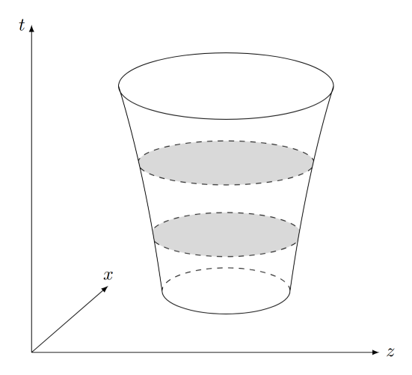
\includegraphics[width=.8\linewidth]{Figures/vaidyanormalslicing.png}
		\caption{The time evolution of the Vaidya black hole slicing for $\alpha = 0$.}
		\label{fig:refnormalslicingvaidya}
	\end{minipage}\hfill
	\begin{minipage}{.46\textwidth}
		\centering
		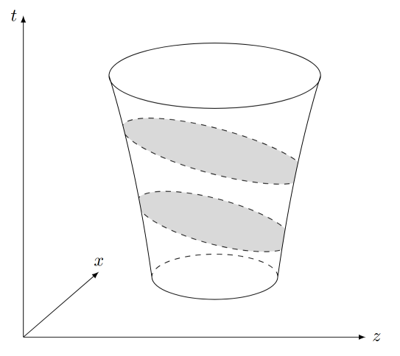
\includegraphics[width=.8\linewidth]{Figures/vaidyafunkyslicing.png}
		\caption{The time evolution of the Vaidya black hole slicing for a nonzero $\alpha$.}
		\label{fig:reffunkyslicingvaidya}
	\end{minipage}
\end{figure}

Looking at the $\alpha = 0$ case in figure \ref{fig:refnormalslicingvaidya}, the MOTSs retain the Vaidya spacetime's spherical symmetry, since the slicing is also spherically symmetric. However, for $\alpha = \frac{10}{11}$ in figure \ref{fig:reffunkyslicingvaidya} this spherical symmetry breaks due to our choice of slicing function $f(z)$. If we had chosen a different slicing function, say $f(x,y)$, this symmetry in the $z$-direction would remain. \newline

We find that there actually is a value for $\tilde{t} < -0.3$ where there are no MOTSs, and it seems to appear suddenly, not growing from a point as we would expect. This can be understood as the 'clipped' bottom of our newly sliced MOTSs, like in figure \ref{fig:vaidyamotssliced}, as the slicing starts to touch the boundary of the MOTSs (the bottom of the cone in figure \ref{fig:reffunkyslicingvaidya}). The reason the south pole is sliced is due to the choice of a positive $\alpha$, if we chose our $\alpha$ to be negative, our slices would be going upwards instead of downwards, clipping the north pole. 

\chapter{Geometric properties of the slicings}

Now that we have found the MOTSs for both Vaidya and Schwarzschild black holes, we actually want to look at the shear and expansion along the MOTSs for both the ingoing and outgoing null vectors. To do that, we perform a spin-weighted spherical harmonic decomposition of the expansion $\theta_{(k)}$ and shear $\sigma_{(k)}$ of the ingoing null normal $k$ as well as the outgoing shear $\sigma_{(\ell)}$ for different slicings: $\alpha=0$  in figure \ref{fig:sph_harmonic_a0.0} and $\alpha = 0.9$ in figure \ref{fig:sph_harmonic_a0.9}. Some further explanation is required for our choice of $\{s,m,\ell\}$\footnote{$\ell$ is now also the degree of our spherical harmonic, as usual.}. We choose $s = 2$ for the shears, since they are spin-2 quantities. Expansion is a spin-0 quantity, so we choose the normal $s = 0$ spherical harmonics. Our starting value of $\ell$ is $|s|$. We therefore start our values of $\ell$ at zero for the expansion, and at two for the shears. Furthermore, in all of our plots, we choose $m=0$. This is due to the fact that, even though we have broken spherical symmetry, axisymmetry still remains.

\begin{figure}[!htb]
	\centering
	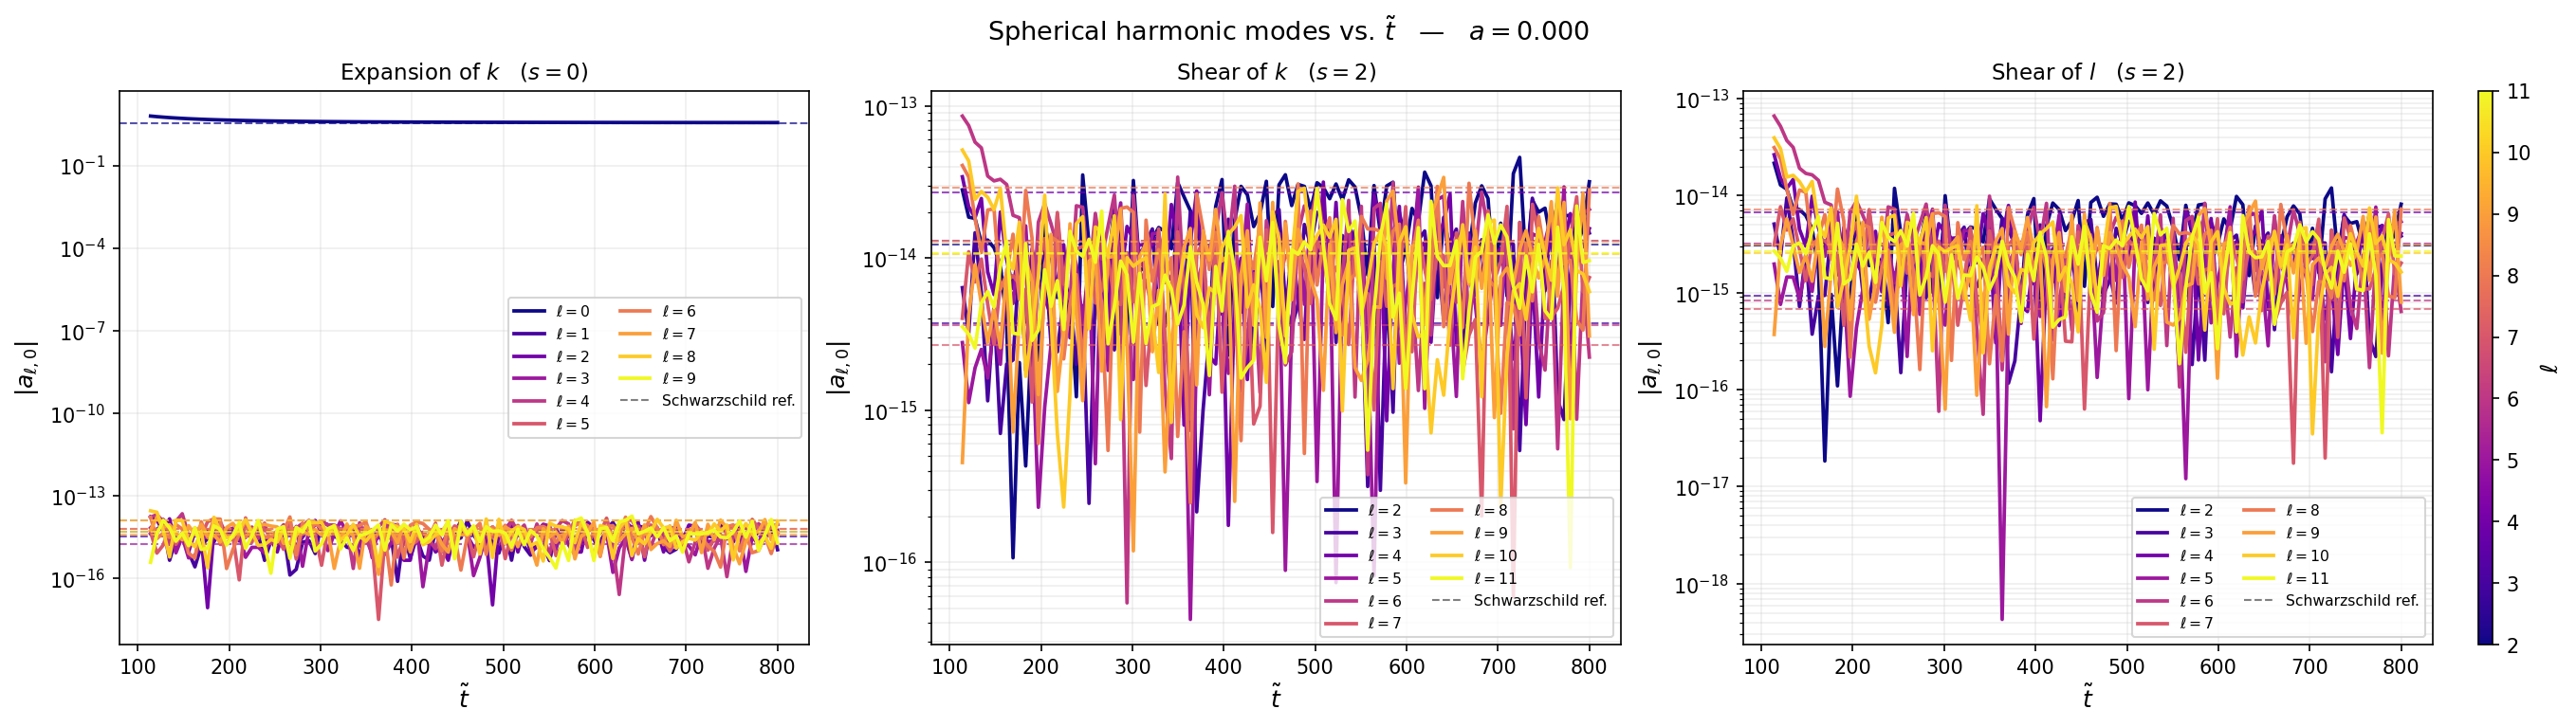
\includegraphics[width=\textwidth]{Figures/Spherical Harmonics/sph_harmonic_a0.000(2).png}
	\caption{This first figure is an decomposition of the ingoing expansion $\theta_{(k)}$ into spin-weighted spherical harmonics, for $s,m=0$, using our normal slicing of $\alpha = 0$. We have performed the same for the ingoing and outgoing shears $\sigma_{(k,\ell)}$, for $s=2$, $m=0$, resulting in the other two figures.}
	\label{fig:sph_harmonic_a0.0}
\end{figure}

Before we go look at the cases for a nonzero $\alpha$, let us study this case more in detail. We plot the strength of each mode of the spherical harmonic over time. First thing to notice in these graphs is to look at the dotted line: we have plotted our results for Schwarzschild here. We would expect, since the Vaidya black hole becomes like a Schwarzschild black hole in the asymptotic future, that both the shear and expansion will converge to our Schwarzschild values at late times. The shears are all of the order of $10^{-14}$ and are thus numerically zero. As can be seen in our figure \ref{fig:sph_harmonic_a0.9}, we can clearly see the convergence to the Schwarzschild case, matching our predictions well. Let us move on to our new slicing in figure \ref{fig:sph_harmonic_a0.9}.\newline
\begin{figure}[!htb]
	\centering
	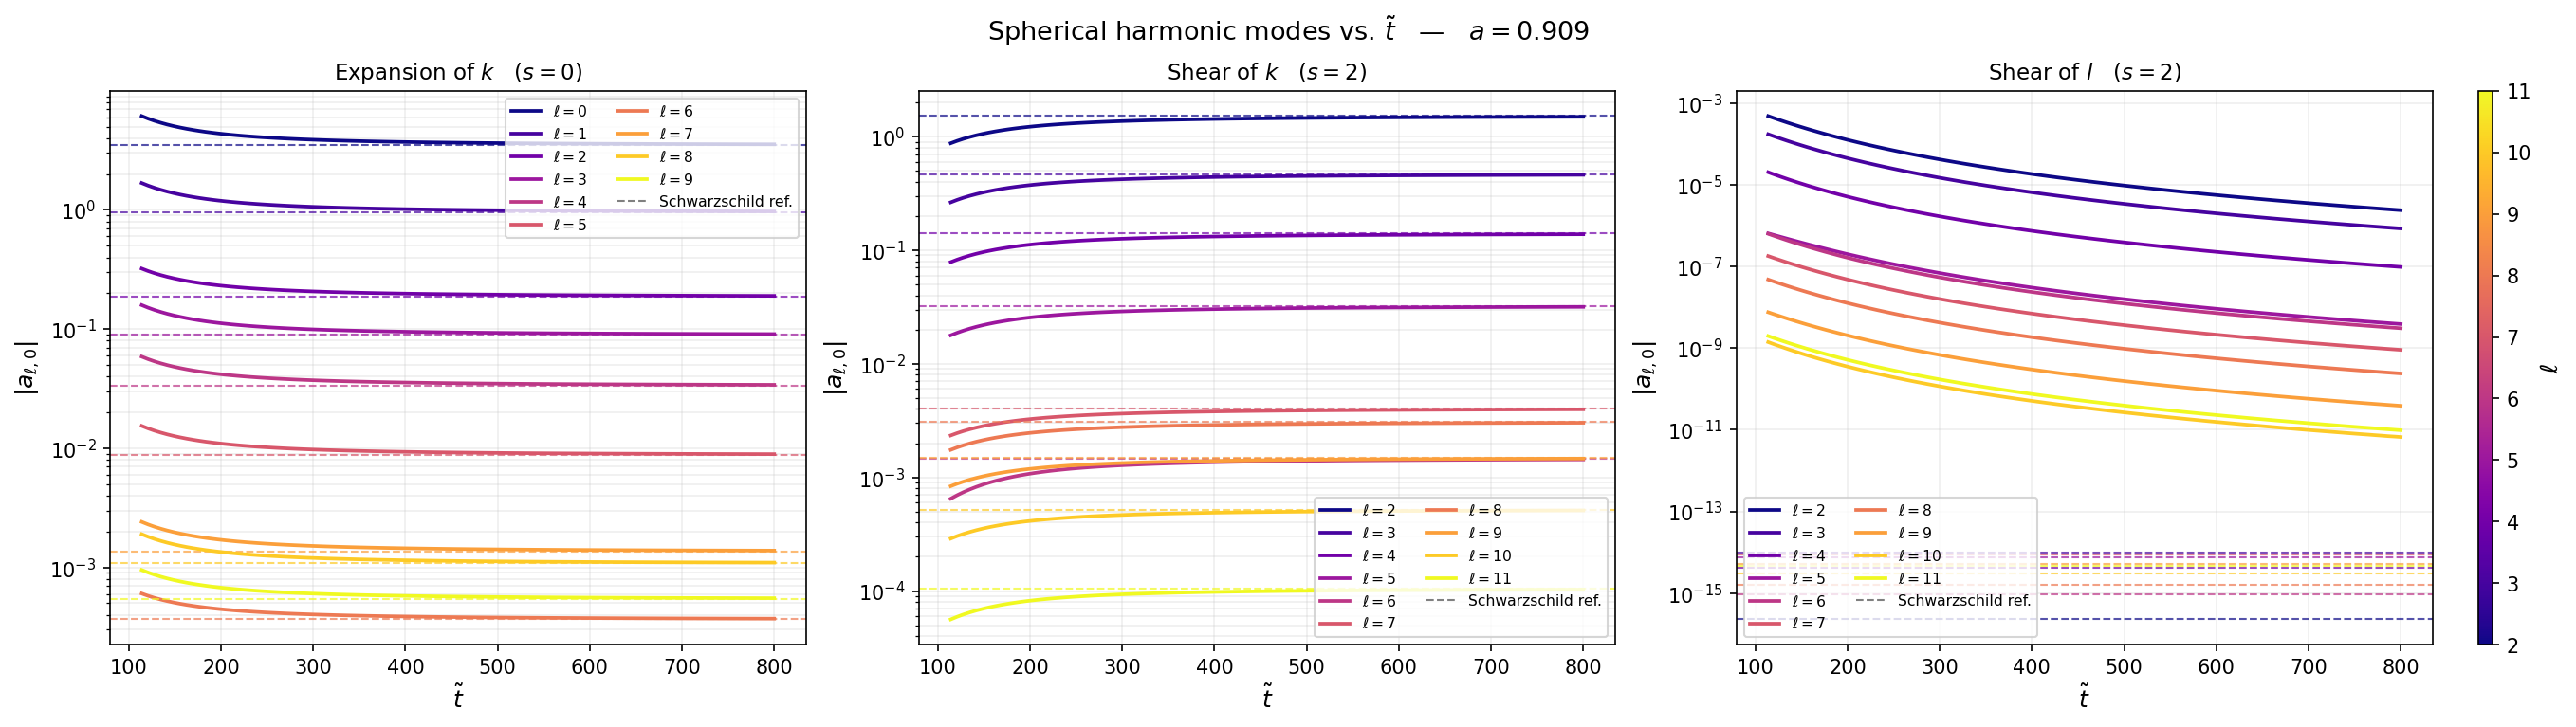
\includegraphics[width=\textwidth]{Figures/Spherical Harmonics/sph_harmonic_a0.909(2).png}
	\caption{Again, this first figure is an decomposition of the ingoing expansion $\theta_{(k)}$ into spin-weighted spherical harmonics, for $s,m=0$, using our new slicing of $\alpha = 0.9$. We have performed the same for the ingoing and outgoing shears $\sigma_{(k,\ell)}$, for $s=2$, $m=0$, resulting in the other two figures.}
	\label{fig:sph_harmonic_a0.9}
\end{figure}

As we can see, once we switch to our new slicing $\tilde{t}$, we get contribution for nonzero $\ell$ in our expansion $\sigma_{(k)}$ and nonzero spherical harmonics to both shears. The asymptotic behavior remains: we recover our Schwarzschild values for higher values of $\tilde{t}$. Most interesting is the fact that the timescale of the outgoing shear $\sigma_{(\ell)}$ returning to the Schwarzschild case is much higher than for the ingoing shear and expansion. \newline

We now want to look back at equation \ref{eq:shearevolution} and see that a changing shear, like in figure \ref{fig:sph_harmonic_a0.9}, implies a nonzero Weyl tensor. This is of our utmost interest, as this could mean the existence of gravitational radiation around the MOTSs is actually dependent on the slicing we use. We do need to be careful with this, as this radiation might just be purely gauge. We will explore this in the next section.


\section{Geometric properties as boosts in Kerr-Schild}

A different way of approaching this problem is found by looking at a paper by Matzner et al. \cite{ksboost}. Here, we can look at a Lorentz boost along an axis to a Kerr-Schild metric. We first look at the general form of Kerr-Schild metrics

\begin{equation}
	ds^2= (\eta_\mn + 2Hk_\mu k_\nu)dx^\mu dx^\nu.
\end{equation}

Here, $H$ is a scalar function, and $k_\mu$ are some null vectors. We now want to figure out what happens to this scalar function $H$ and its corresponding null vectors as we boost them in some direction. The Minkowski part of the metric stays the same, as it is boost-invariant. Looking at the more specific Schwarzschild case, we recall its Kerr-Schild form as

\begin{equation}
	ds^2 = -dt^2 + dx^2+dy^2+dz^2+\frac{2M}{r}(dt+dr)^2,
\end{equation}

\newpage
we now perform a Lorentz boost in the $z$-direction with velocity $u$, using primes for boosted coordinates:

\begin{equation}
	t' = \gamma(t+uz), \quad z' = \gamma(z+ut), \quad x' = x, \quad \text{and} \quad y' = y.
\end{equation}

We arrive at the following metric:

\begin{equation}
	ds^2 = -dt'^2 + dx'^2 +dy'^2 + dz'^2+\frac{2M}{r}\left(\gamma(dt'-udz')+ dr\right)^2.
	\label{eq:boostedschwarzschild}
\end{equation}

Where $r$ also obtains an explicit time dependence, with $r^2 = x^2 + y^2 + \gamma^2(z' - ut')^2$. We now start to calculate our $k_{\mu'}$, defined as $k_{\mu'} = \frac{\partial x^\alpha}{\partial x^{\mu'}}k_\alpha$, transforming like we expect a (0,1)-tensor to transform :

\begin{equation*}
	k_{t'} = \gamma(1-\gamma u\frac{z'-ut}{r})
\end{equation*}

\begin{equation*}
	k_{z'} = \gamma(-u+\gamma \frac{z'-ut}{r})
\end{equation*}

\begin{equation*}
	k_{x'} =\frac{x'}{r}
\end{equation*}

\begin{equation*}
	k_{y'} =\frac{y'}{r}
\end{equation*}


where, following Matzner et al. \cite{ksboost}, $k_i$ can be defined as

\begin{equation}
	k_i = \partial_i\frac{M}{H}-\gamma u_i.
	\label{eq:boostedkscorrections}
\end{equation}

With some algebra, we can show that this is the case. This boost can be thought of as 'tilting' our time axis, much like we have done during our slicing of the Schwarzschild metric. This motivates us to look at the Vaidya case and maybe gain an explanation for our gauge issues. 

\subsection{Vaidya slicing as boosted Kerr-Schild metrics.}

For this, we return to the ingoing Vaidya metric in Kerr-Schild coordinates (equation \ref{eq:vaidyametrickerrschild}):

\begin{equation*}
	ds^2 = -dt^2 + dx^2+dy^2+dz^2+\frac{2M(t+r)}{r}(dt+dr)^2,
\end{equation*}

This is, of course, the same as the Schwarzschild example, albeit with a promoted mass function. We will again boost this metric in the $z$-direction with a velocity $u$ and achieve the same result.

\begin{equation*}
	ds^2 = -dt'^2 + dx'^2+dy'^2+dz'^2+\frac{2M(v')}{r}\left(\gamma(dt'-udz')+ dr\right)^2
\end{equation*}


where $v' = t' + r$ is our boosted Vaidya time. We now want to recall the sliced Vaidya metric from section 3.3.2:

\begin{equation}
	ds^2 = -(d\tilde{t} - f'(z)dz)^2 + dx^2 + dy^2+ dz^2 +\frac{2M(\tilde{v})}{r}(d\tilde{t} - f'(z)dz+dr)^2.
\end{equation}
\newpage

\noindent Expanding the first term, we arrive at 

\begin{equation}
	ds^2 = -d\tilde{t}^2 + 2f'(z)d\tilde{t}dz + dx^2 + dy^2+ (1-f'(z)^2)dz^2 +\frac{2M(\tilde{v})}{r}(d\tilde{t} - f'(z)dz+dr)^2
\end{equation}

with $\tilde{v} = \tilde{t} - f(z) + r$ our sliced Vaidya time.\newline

Of course, these two 4-metrics are trivially the same geometry, as we have only performed two different coordinate transformations on the same metric. We have only rescaled the time and space coordinates on each slice of our ADM-spacetime, as we can see in the difference of shift $N_i$ and lapse $N$. We can think of the slicing transformation as purely the temporal part of the Lorentz boost, thus causing the two metrics to differ while describing the same geometry. However, restricting ourselves to the MOTSs, the boost and non-standard time slicing may turn out to be equivalent, providing us with an argument for our apparent 'radiation'.

\subsection{Matching boosted foliations to the slicing function}

The boosted and sliced time coordinates do look extremely similar, matching if we set $f'(z) = u$, or more explicitly, 

\begin{equation}
	f(z) = uz + C
	\label{eq:transformation}
\end{equation} 

where $C$ is an arbitrary constant. It is important to mention we have restricted ourselves to linear slicing functions.  We want to look at the hypersurfaces created by these foliations, as these MOTS live on a hypersurface. Using equation \ref{eq:transformation}, we can create a transformation $\Phi$ between the boosted and sliced metrics:

\begin{equation}
	\Phi: \quad t' = \gamma \tilde{t}, \quad \text{and} \quad z' = \frac{z}{\gamma} + \gamma u \tilde{t},
\end{equation}

we find that our $t'$ and $\tilde{t}$ actually only differ by a scalar factor $\gamma$. This means that only the threading between the hypersurfaces is different: the hypersurfaces themselves are identical. Trivially, we can then say that the MOTSs also match. If we want to convince ourselves a bit more, we can explicitly calculate this and see that the metrics match. \newline

Rearranging $\Phi$, we get $z = \gamma(z' - ut')$, the temporal term added to $r$ due to the Lorentz boost. Similarly, we can use this transformation to show that these 3-metrics match, starting with the $\gamma(dt' -udz')$ term:

\begin{equation}
	\begin{split}
		\gamma(dt' -udz') = \\
		\gamma(\gamma d\tilde{t} - \frac{u}{\gamma}dz - \gamma u^2dT) =\\
		\gamma^2d\tilde{t} - udz - \gamma^2 u^2 dT =\\
		d\tilde{t} - udz = d\tilde{t} - f'(z)dz.
	\end{split}
\end{equation}

The $dt'$ and $dz'$ terms also coincide using the same logic:

\begin{equation}
	\begin{split}
		-dt'^2+dz'^2 =\\
		-\gamma^2d\tilde{t}^2+\frac{1}{\gamma^2}dz^2 + 2ud\tilde{t}dz + \gamma^2 u^2d\tilde{t}^2=\\
		-d\tilde{t}^2 + 2ud\tilde{t}dz + (1-u^2)dz^2.
	\end{split}
\end{equation}

Finally, the boosted and tilted Vaidya times also match:
\begin{equation}
	\begin{split}
		v' = \gamma(t'- uz')+r =\\
		\gamma^2(1-u^2)\tilde{t}-uz+r = \tilde{t} - f(z)+r =\tilde{v}
	\end{split}
\end{equation}

We find that these foliations match each other, even if the lapse and shift do not agree. This is because the shift and lapse only describe the motion between hypersurfaces. Therefore, we can say that the induced metric and extrinsic curvature for both of these foliations are the same (and therefore the MOTSs!), under a transformation $\Phi$. We can now confidently think of $\alpha$ as being equal to our boost velocity $u$ and look at its gauge effects on the shear we observe.

\section{Gauge radiation in boosted Vaidya metrics}

We now try to explain why this boosted Vaidya metric coinciding with our sliced metric describes our gauge gravitational radiation. As we have discussed, we can search for this radiation by measuring the Weyl tensor. Using private notes from dr. B. Bonga based on a paper by Booth and Fairhurst in 2007 \cite{Booth_2007},  we can find that our $\alpha$ corresponds to a normal deformation of the standard $t$ slicing by

\begin{equation}
	X^a = Ak^a- Bn^a,
\end{equation}

with 

\begin{equation}
	\begin{split}
		A_0 = 3r_0\frac{\cos\theta}{3-2\dot{M}(v)}, \\
		B_0 = 2r_0\frac{\dot{M}(v)\cos\theta}{3-2\dot{M}(v)}
	\end{split}
\end{equation}

which is an $\ell = 1$ dipole at leading order in $\alpha$.\newline

Here, $r_0 = 2M_0$ is the unperturbed radius of the MOTS. Looking at the Schwarzschild case, where $M$ is a scalar, $\dot{M} = 0$, $X^a$ becomes $zk^a$, which is null. Therefore the MOTS is unchanged, supporting our conclusion from chapter 3. For the Vaidya case, the MOTSs are spacelike, so we get an actual change in $k^a$. Using this insight, one can also show that the shear at leading and linear order in $\alpha$ has to be zero and only at order $\alpha^2$ starts to become non-zero with its analytic expression given by

\begin{equation}
	\sigma_{ab}^{(\ell)}|_{\mathcal{O}(\alpha^2)} = \frac{\alpha^2}{2}\left[-\beta_2D_{\langle a}D_{b\rangle}P_2(\cos\theta)-A_0\tilde{q}^e_{\hphantom{a}a}\ell^d\tilde{q}^e_{\hphantom{a}b} \ell^fC_{cdef}|_{\mathcal{O}(\alpha^2)} + ... \right]
\end{equation}


Now, at small $\alpha$, we can approximate $\|\sigma^{(\ell)}\| \propto \alpha^2$. Of course, we can check this within MOTSfinder and arrive at figure \ref{fig:shearvsalpha}

\begin{figure}[!htb]
	\centering
	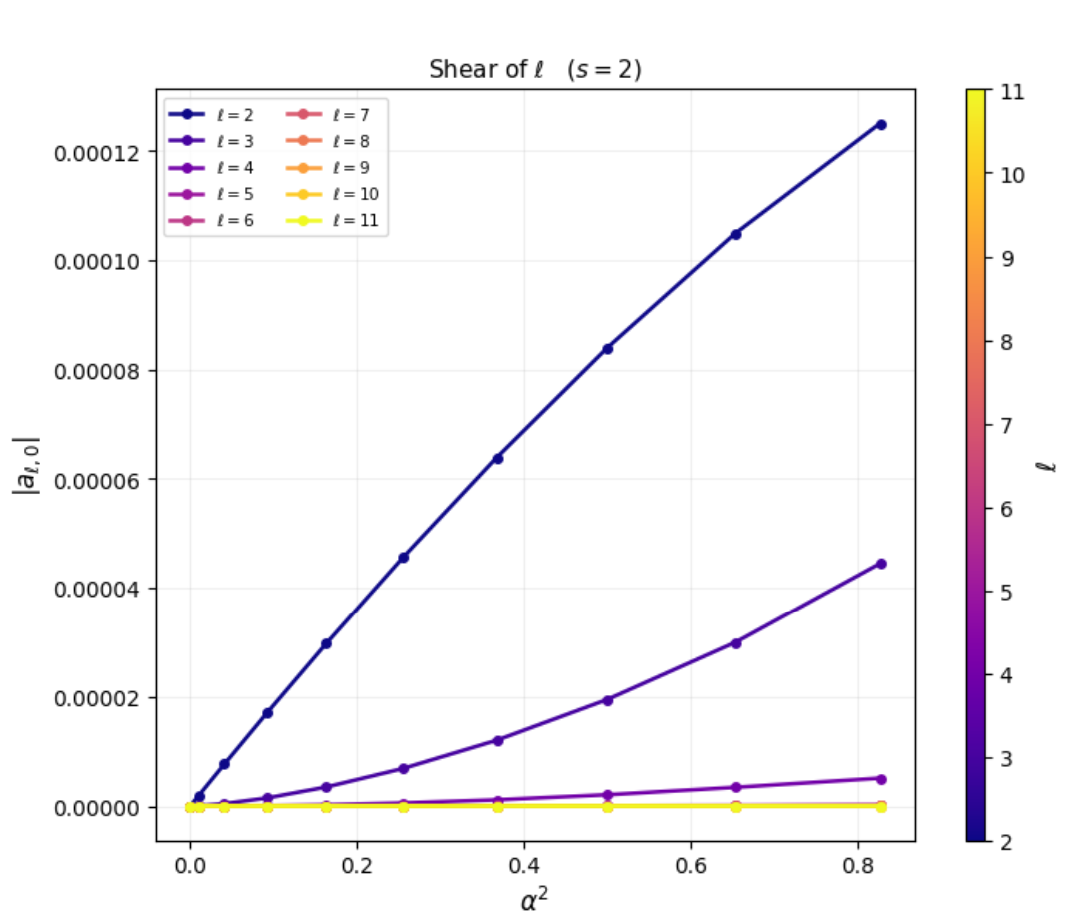
\includegraphics[width=0.8\textwidth]{Figures/shearl}
	\caption{Simulations for the $\alpha$-dependency of our outgoing shear $\sigma_{(\ell)}$.}
	\label{fig:shearvsalpha}
\end{figure}

As we can see, the $\ell = 2$ mode (the darkest blue line) for small values of $\alpha^2$ looks linear, confirming our suspicion. For higher values of $\alpha^2$, other modes of $\ell$ start to become relevant. Nonetheless, our claims hold. The gravitational 'radiation' we see in figure \ref{fig:sph_harmonic_a0.9} is nothing more than gauge, which can be explained by reinterpreting the slicing of the spacetime as a Lorentz boost. 


\chapter{Discussion and interpretation}

\section{Issues with computation time}

Most issues with this research reside in the numerical nature of the study. As we have discussed in previous sections, runtime issues with the Vaidya spacetime do not provide us with the opportunity to always check the validity of our spacetimes as rigorously as we would want to. For our cases, we had some literature to fall back upon, but this will not always be the case. We will therefore need to be careful with using Mathematica to slice our different metrics. \newline

MOTSfinder has some of the same issues. Computations for finding MOTSs for about 10 values of $\alpha$, for about 100 $\tilde{t}$-values takes a considerable amount of computation time (approx. 8 hours) on a local laptop (using a Ryzen AI 7 350 CPU with 32 GB's of RAM), this hampers the ability to quickly check some MOTSs, slowing down some research. Making use of the \verb*|cython| package might allow us to speed everything up. Of course, this is only necessary for the first couple runs of MOTSfinder with a new metric, as we need to find suitable values for $t$ and $\alpha$ to clearly illustrate the slicing-dependent properties. We also need a many values of $t$ to look at the expansion into spherical harmonics (generating figures \ref{fig:sph_harmonic_a0.0} and \ref{fig:sph_harmonic_a0.9}). \newline

Nonetheless, we see that MOTSfinder is able to adequately predict MOTSs found using other methods in the literature. This motivates us to start looking at more complex metrics in the future. It seems clear that this method has a lot of potential for further research.

\section{Outlook}


\subsection{Relating Lorentz boosts to slicings}
More research into the slicing-dependent geometric properties of MOTSs has the potential to provide us with more insight. By relating linear slicings of the Vaidya and Schwarzschild spacetimes to Lorentz boosts, we have found more familiar language to explain possible gauge issues, thus making these methods more reliable in the long term. \newline

Expanding this reasoning into more complex spacetimes, such as Kerr-Vaidya, might allow us to reach the same conclusion or find some new gauge issues to tackle, to further our knowledge on this specific area of numerical relativity. \newline

Of course, different slicings may prove to show different results, as we can add more multipole terms to the slicing to see what happens to our MOTSs. We have only shown correspondence between linear slicings and Lorentz boosts, but it might be possible to relate multipole slicings to a different diffeomorphism. 

\subsection{Gauge radiation}

In-depth research into the effect of slicing on the Weyl scalars is beyond the scope of the thesis, but might prove to be interesting. When using MOTSfinder to find MOTSs emitting radiation in numerical pieces of a metric, we should first explore the possibility that this is pure gauge.\newline

In general, the arguments set forth in this thesis could be recast into a more elegant form by using the framework of group theory, allowing us to formulate our conclusions with much more mathematical rigour.\newline

We conclude by noting that extending all of this research into numerical metrics or non-asymptotically flat metrics might prove to give us some exciting new results.

\section{Acknowledgments}

I would foremost like to thank my supervisor, dr. Béatrice Bonga, for creating this wonderful research opportunity and guiding me in a way that made the research and writing extremely fun and illustrative. Furthermore, I thank prof. dr. Badri Krishnan for not only being the second assessor, but also for suggesting several papers pointing this research in the right direction. Finally, I would like to thank Anna van Asselt, MSc, for contributing some incredibly useful comments regarding the Mathematica and MOTSfinder parts of this thesis. 



\appendix
\chapter{Research data management}
\label{chapter:rdm}
All code to reproduce these results, including the classes for the different metrics, can be found in the following GitHub repository: \textcolor{cyan}{\url{ https://github.com/RvanWitzenburg/Bachelorthesis_VaidyaMOTS}}.

\newpage
\printbibliography[heading=bibintoc]

\end{document}
